%%%%%%%%%%%%%%%%%%%%%%%%%%%%%%%%%%%%%%%%%%%%%%%%%%%
%
%  New template code for TAMU Theses and Dissertations starting Fall 2012.  
%  For more info about this template or the 
%  TAMU LaTeX User's Group, see http://www.howdy.me/.
%
%  Author: Wendy Lynn Turner 
%	 Version 1.0 
%  Last updated 8/5/2012
%
%%%%%%%%%%%%%%%%%%%%%%%%%%%%%%%%%%%%%%%%%%%%%%%%%%%
%%%%%%%%%%%%%%%%%%%%%%%%%%%%%%%%%%%%%%%%%%%%%%%%%%%%%%%%%%%%%%%%%%%%%%
%%                           SECTION IV
%%%%%%%%%%%%%%%%%%%%%%%%%%%%%%%%%%%%%%%%%%%%%%%%%%%%%%%%%%%%%%%%%%%%%

\chapter{\uppercase{Implementation}}
To solve the problems stated in pevious chapters, we develop seismic analytics cloud platform (SAC for short). The goal of SAC is to deliver a scalable and productive cloud Platform as a Service (PaaS) to seismic data analysis researchers and developers. SAC has two main characteristics: one is able to process big data and another is easy to use for geology domain experts. With SAC, user only need focus on data analytics logic itself without caring about details on data storage and computing model. 

%SAC is designed to be able to store large amount of seismic data with major vendor's formats, as well as be able to process them in the scalable fashion to meet the performance requirements. Users should be able to work on their seismic processing algorithms using high-level programming models with very limited knowledge in parallelism and architecture.

\section{Architecture}

In the beginning, the mainframe is widely used for seismic data processing and each job regardless of running time needs to be put into queue waiting for execution. With the improvement of CPU power, more softwares were transfered to personal coputer(PC) for better portibility and interactivity. But with the growth volume size of sesimic data, frequence of single core could not increase limitless and scalable resources are need to handle variable requirements, more and more softwares are then moved to cloud platform by utilizing parallelization dynamically. Such trend brings big change on business model: from selling software lisence to charging for service. In clould platform, the thin client could request storage and computation resources basing on requirement, and in such way whole cluster or huge data center could be used efficiently. In HPC domain, MPI or PVM could also build on cluster, which fully utilize all resources in whole cluster but need deep understanding of data distributation and communication. The data storage in HPC is typical using centralized storage manager with disk array, which needs data movement between storage nodes and worker nodes. To overcome problems of HPC, we build SAC as service with template-based programming interface on cloud platform, and to make it easy to use, some popular image processing and signal processing software packages are integrated into SAC.  

Figure \ref{SACSWStack} shows the overall software stack used in SAC. In this diagram, the operating systems at 1st level from bottom to top could be Unix-like or Windows system running on virtual machine or bare metal. Above the OS layer, there should be a layer provides compiling and running environment, which include JRE\/JDK, Scala, Python and other native libraries such as OpenCV, FFTW etc. Java has already became the dominating language in application development for its cross-platform and simplicity \cite{Top10Lang}. Scala is a new general-purpose programming language that support both object\-oriented and functional programming language but still runs on JVM and is compatible with existing Java libraries. Most big data processing platform such as Hadoop, Storm, HBase and Cassandra etc. are written in Java and provide Java programming inerfaces; Spark is developed in Scala itself but applications running on it could be developed in Java, Scala or Python. For the performance issue, some computation intense libraries such FFTW and OpenCV are written in C++, but they also provide Java interface through JNI that could be used on JVM. In third layer, there are some common componets installed including HDFS, Mesos and YARN  used for data storage and resource scheduling. HDFS is distributed file system delivered in Hadoop that provides highly fault-tolerance and high throughput access to big data set. In SAC, HDFS is used for storing original binary seismic data. The metadata and intermediate data such as seismic attribute are stored in Cassandra database. Resource management in cluster is very important for job scheduling and load balance, and in SAC, Standalone, Mesos and YARN are all supported. In the fourth layer from bottom, it includes the actual computation components: signal and image processing libraries with Java/Scala interface; Breeze \cite{ScalaNLPBreeze} is a set of libraries for machine learning and numerical computing written in Scala and Java. FFTW \cite{Frigo05thedesign} is a C subroutine library for computing the discrete Fourier transform (DFT) with one or more dimensions in both real and complex data format. There are already some Java FFTW wrappers make it could be used on JVM without giving up performance. SAC chose Spark as computation platform due to its performance achieved with in\-memory computation and its fault tolerance. The main work of this paper are focus on second and third layer from top. Seismic Applications are mainly developed by end users. Seismic Analytics Cloud layer is used for providing SDK and running environment for client applications. Template-Based framework provides common programming models for domain specific experts, and workflow could connect piece of algorithms or models into a job chain as well as run it automatically. Visualization is important for user to view results and generate useful information intuitively.  

%The design of SAC architecture is to emphasize twofold: one is to provide a high-level productive programming interface to simplify the programming efforts; the other is to execute user's applications with scalable performance. To achieve the first goal, we provide the web interface in which user could manage seismic datasets, programming within a variety of templates, generate complete source codes, compiling and then running the application and monitoring the job running status in SAC. 

%The interface allows users to write seismic data processing algorithms using our extracted common seismic computation templates, which lets users focus on their kernel algorithm implementation, and simplifies user's implementation in handling seismic data distribution and parallelism. 
%While the most popular-used programming models in seismic data processing include MATLAB, Python, C/C++, Fortran, Java and more, SAC supports Java, Python and Scala natively, so that users can write their own processing algorithms directly on our platform with these three languages; For legacy applications written in other languages, SAC uses the so-called PIPE mode to handle input and output data as standard-in and -out, which requires minor modifications of program source code on handling input and output. 
%SAC will generate complete Spark codes based on user's kernel codes and configurations, and then launch and monitor it on the SAC environment.
In order to support large amount data storage and scalable I/O performance, we chose Hadoop HDFS as the underlying file system, which provides fault tolerance with duplicated copies and good I/O throughput by supporting data locality information to applications. HDFS supplies out-of-the-box redundancy, failover capabilities, big data storage and portability. Since the size of seismic data is very large and keeps increasing constantly, HDFS provides a good solution for the data storage with fault tolerance property.

%We use Spark as the parallel execution engine to start applications, since Spark works well on top of HDFS, Mesos [13] and YARN, and it provides a big data analytics computing framework with both in-memory and fault-tolerance support. Spark provides RDD as a distributed memory abstraction that lets programmers perform in-memory computations on large-scale cluster/cloud in a fault-tolerant manner. To get better performance, we need to put frequently used data into memory and processing data in memory, which is one key performance boost comparing with MapReduce.Some other useful packages and algorithms in data analytics, such as SQL, machine learning and graph processing, are also provided in Spark distribution version. We also integrated some common used libraries for image processing and signal processing, such as OpenCV, Breeze and FFTW etc., to provide a rich third party of libraries support to speed up the development process. Figure \ref{SACSWStack} shows the overall software stack used in SAC.

Figure \ref{SACArch} presents the overall architecture of SAC. Based on the SAC web interface, Users are able to upload, view and manage their seismic data, which are stored on HDFS. They can then create their application projects by selecting a template from a list of predefined templates to start their own programming. After selected dataset and processing pattern, writing codes and compiling successfully, users can configure the running parameters and then submit jobs to SAC. Job status could be monitored while job is running and running results could be checked after job is finished. On the SAC backend, a big seismic data file will be split into multi-partitions and be constructed into RDD, which will be processed by working threads that apply user's algorithm in parallel. After all data are processed, the output data will be saved back to HDFS.

%%%%%%%%%%%%%%%%%%%%%%%%%%%%%%%%%%%%%%%%%%%%%%%%%%%%%%
\begin{figure}[H]
\centering
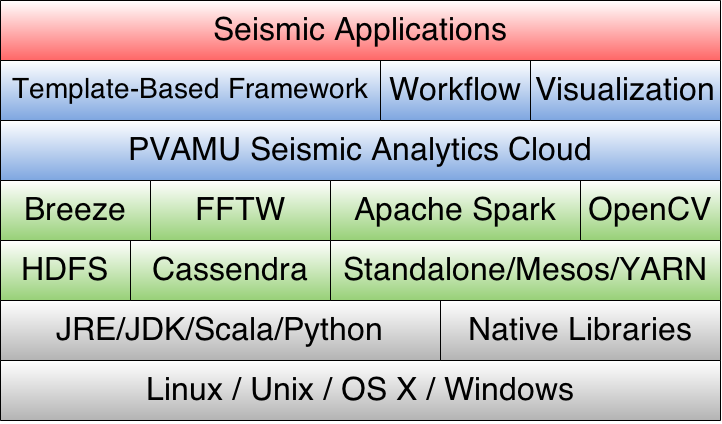
\includegraphics[scale=.50]{figures/SACSWStack.png}
\caption{The Software Stack of Seismic Analytics Cloud Platform}
\label{SACSWStack}
\end{figure}
%%%%%%%%%%%%%%%%%%%%%%%%%%%%%%%%%%%%%%%%%%%%%%%%%%%%%%

%%%%%%%%%%%%%%%%%%%%%%%%%%%%%%%%%%%%%%%%%%%%%%%%%%%%%%%
\begin{figure}[H]
\centering
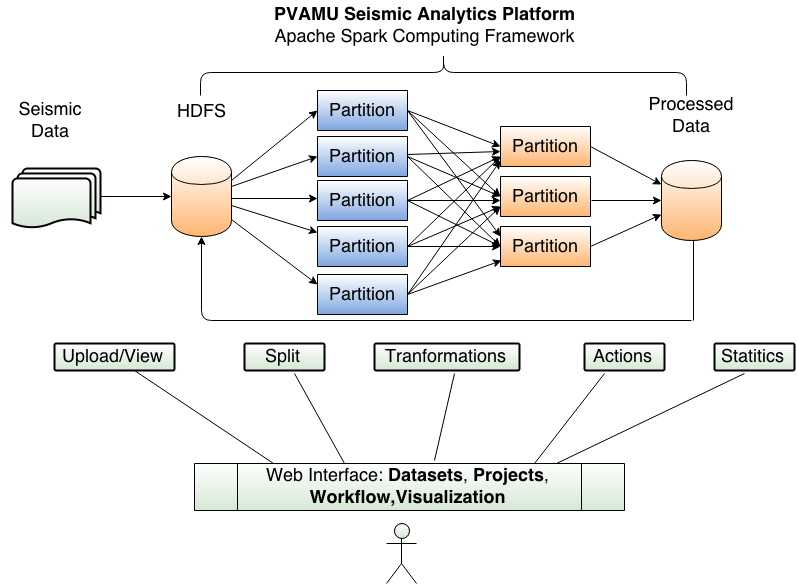
\includegraphics[scale=.50]{figures/SACArch.png}
\caption{The Architecture of Seismic Analytics Cloud Platform}
\label{SACArch}
\end{figure}
%%%%%%%%%%%%%%%%%%%%%%%%%%%%%%%%%%%%%%%%%%%%%%%%%%%%%%%

\section{Data Storege and Distribution}

The SEG Y (also SEG-Y) \cite{} file format is one of several standards developed by the Society of Exploration Geophysicists (SEG) for storing geophysical data. This kind of big seismic data needs to be split into multiple small partitions to be processed in parallel. However, SEG Y data could not be split directly due to its irregularity, so we preprocess the SEG Y data format into a regular 3D volume data, and store the important header information into one xml file. Then the 3D volume data and xml will be feed into Spark applications. Spark uses InputFormat, which is the base class inherited from Hadoop to split such data and construct RDD. Each split will be mapped to one partition in RDD. The embedded InputFormat classes could not handle binary seismic data, so we implemented SeismicInputFormat in this project.  Based on configuration defined by user while creating project, such as how many lines each split and number of overlap lines, SeismicInputFormat could spilt the 3D volume and feed partition to each mapper. The data of 3D volume is stored trace by trace in the Inline direction by default. For some algorithms that need to process data in cross-line or time-depth direction, we also provide interfaces to transform Inline format RDD into cross-line or time-depth direction. In this way, we could cache Inline format RDD in memory, thus all the transformations could be executed in memory with better performance.

%\begin{table}[H]
%\centering
%\caption{This is a table template}
%\begin{tabular}{|l|c|c|c|c|c|}
%\hline
%Product & 1 & 2 & 3 & 4 & 5\\
%\hline
%Price & 124.- & 136.- & 85.- & 156.- & 23.-\\
%Guarantee [years] & 1 & 2 & - & 3 & 1\\
%Rating & 89\% & 84\% & 51\% & & 45\%\\
%\hline
%\hline
%Recommended & yes & yes & no & no & no\\
%\hline
%\end{tabular}
%\label{tab:template2}
%\end{table}


\section{Template}

Based on the general parallel execution patterns of seismic processing algorithms and applications, we predefined some templates to make this framework easy to program. Every template has explicit input type and output type. The typical templates are: Pixel pattern, which use sub-volume or one pixel as input and output one pixel; Line pattern, which treat one line as input and one line as output; SubVolume pattern, which feed user’s application with sub-volume and get output from it in sub-volume format. A high level SeismicVolume class has been implemented in this project to provide user interface to access seismic volume. SeismicVolume class provides functions for constructing RDD based on processing templates user had selected, applying user's algorithms on RDD, and storing the final RDD on HDFS with format defined by user. To make it easy for programming, we provide some other functions to change the linear array into 2D matrix and 3D volume class; some functional programming interface such as iteration, map/flatMap, filter and zip could be used. We also integrated commonly used high-level algorithms, such as histogram, FFT, interpolating and filtering algorithms, so that user could put more attention on data analytics logic instead of details for each algorithm.

\section{Seismic RDD}


\section{Code Generator}

After user created project and completed their own kernel codes, one component named Code Generator (CG) in SAC will generate complete Spark codes for running on Spark platform. The CG will parse configuration of user's project and generate Spark application outlined codes, merge them with user's codes. User could also upload existing source codes or libraries, all of which will be integrated into current working project managed by Simple Build Tool (SBT). CG will also generate compiling and running scripts basing on user's runtime setting. All these scripts will be called by the web interface, on which some other information such as compiling and running status, location of output will be shown clearly.

\section{Application Executation}

In SAC, every user's project will be treated as one Spark application. CG will generate the main driver code for each project. Each application could be submitted to SAC for running after compiled successfully. At execution time, driver code will setup the Spark running time environment, call the SeismicVolume object to generate RDD and execute user's algorithms on top of RDD and then store the processed results on HDFS. It will clean up the running environment and release resources after finished. To make it support multiple users, Spark Jobserver \cite{}  was introduced to this platform. Based on the priority of application and computation resources requirement of an application, an user could configure the running parameters: number of cores and memory size; and then submit his/her own job, monitoring job status and viewing the running results. Another big advantage of Spark Jobserver is supporting of NamedRDD that allows multiple applications share RDD but has only one copy cached in memory. For some complicate algorithms that need multiple steps or application running in workflow, NamedRDD is a good choice for boosting performance. After job is finished, the running results cloud be discarded or be saved to user's workspace basing on user's selection.

